\documentclass{article}[11pt]
\textheight 8.5in
\usepackage{graphicx}
\usepackage{float}%for forcing position of figs
\usepackage{hyperref}
\usepackage{url}
\usepackage{comment}

\usepackage{amsmath}
\usepackage{amsthm}

\usepackage{amssymb}
\usepackage{bm}

%%%%%%%%%%%%%%%%%%%%%%%%%%%%%%%%%%%%%%%%%%%%%%%%%%%%%%%%%%%%%%%%%%%%%%%%%%%%%%%%
% based on defs.tex by S. Boyd
% modified by Jie Fu
\newif\ifuseboldmathops
\newif\ifuseittextabbrevs
\useboldmathopstrue   % comment out to use mathbb
%\useittextabbrevstrue % comment out to use non-italic text abbrevs like e.g.
%%%%%%%%%%%%%%%%%%%%%%%%%%%%%%%%%%%%%%%%%%%%%%%%%%%%%%%%%%%%%%%%%%%%%%%%%%%%%%%%

% text abbrevs
\ifuseittextabbrevs
	\newcommand{\cf}{{\it cf.}}
	\newcommand{\eg}{{\it e.g.}}
	\newcommand{\ie}{{\it i.e.}}
	\newcommand{\etc}{{\it etc.}}
	\newcommand{\etal}{{et~al.}}
\else
	\newcommand{\eg}{e.g.}
	\newcommand{\ie}{i.e.}
	\newcommand{\etc}{etc.}
	\newcommand{\etal}{et~al.}
\fi

% standard math sets
\ifuseboldmathops
	%\newcommand{\reals}{{\mbox{\bf R}}}
	\newcommand{\reals}{\mathbf{R}}
	\newcommand{\integers}{\mathbf{Z}}
	\newcommand{\complex}{\mathbf{C}}
	\newcommand{\symm}{\mathbf{S}}  % symmetric matrices
\else
	\newcommand{\reals}{\mathbb{R}}
	\newcommand{\integers}{\mathbb{Z}}
	\newcommand{\complex}{\mathbb{C}}
	\newcommand{\symm}{\mathbb{S}}  % symmetric matrices
\fi

% control theory sets
\ifuseboldmathops
	\newcommand{\HH}{\mathbf{H}}
	\newcommand{\LL}{\mathbf{L}}
\else
	\newcommand{\HH}{\mathbb{H}}
	\newcommand{\LL}{\mathbb{L}}
\fi

% probability operators
\ifuseboldmathops
	\newcommand{\Expect}{\mathop{\bf E{}}\nolimits}
	\newcommand{\Prob}{\mathop{\bf P{}}\nolimits}
\else
	\newcommand{\Expect}{\mathop{\mathbb{E}{}}\nolimits}
	\newcommand{\Prob}{\mathop{\mathbb{P}{}}\nolimits}
\fi

% convex operators
\ifuseboldmathops
	\renewcommand{\Re}{\mathop{\bf Re}}
	\renewcommand{\Im}{\mathop{\bf Im}}
	
	\newcommand{\prox}{\mathop{\bf prox}} % proximal operator
	\newcommand{\dom}{\mathop{\bf dom}}   % domain
	\newcommand{\aff}{\mathop{\bf aff}}   % affine hull
	\newcommand{\cl}{\mathop{\bf cl}}     % closure
	\newcommand{\intr}{\mathop{\bf int}}  % interior
	\newcommand{\Co}{\mathop{\bf Co}}     % convex hull
	\newcommand{\relint}{\mathop{\bf rel int}} % relative interior
	\newcommand{\bd}{\mathop{\bf bd}}     % boundary
	
	\newcommand{\Tr}{\mathop{\bf Tr}}
	\newcommand{\diag}{\mathop{\bf diag}}
\else
	\renewcommand{\Re}{\mathop{\mathrm{Re}}}
	\renewcommand{\Im}{\mathop{\mathrm{Im}}}
	
	\newcommand{\prox}{\mathop{\mathrm{prox}}} % proximal operator
	\newcommand{\dom}{\mathop{\mathrm{dom}}}   % domain
	\newcommand{\aff}{\mathop{\mathrm{aff}}}   % affine hull
	\newcommand{\cl}{\mathop{\mathrm{cl}}}     % closure
	\newcommand{\intr}{\mathop{\mathrm{int}}}  % interior
	\newcommand{\Co}{\mathop{\mathrm{Co}}}     % convex hull
	\newcommand{\relint}{\mathop{\mathrm{rel int}}} % relative interior
	\newcommand{\bd}{\mathop{\mathrm{bd}}}     % boundary
	
	\newcommand{\Tr}{\mathop{\mathrm{Tr}}}     % trace
	\newcommand{\diag}{\mathop{\mathrm{diag}}} % diagonal matrix
\fi

% useful non-bold operators
\newcommand{\eqbydef}{\mathrel{\stackrel{\Delta}{=}}}
\newcommand{\eqbyset}{\mathrel{\stackrel{\mathrm{set}}{=}}}
\newcommand{\argmax}{\mathop{\mathrm{argmax}}}
\newcommand{\argmin}{\mathop{\mathrm{argmin}}}

% lin alg stuff
\newcommand{\Span}{\mathop{\mathrm{span}}}
\newcommand{\Range}{\mathop{\mathrm{range}}}
\newcommand{\Null}{\mathop{\mathrm{null}}}
\newcommand{\rank}{\mathop{\mathrm{rank}}}

\newcommand{\ones}{\mathbf 1}
\newcommand{\lambdamax}{{\lambda_{\rm max}}}
\newcommand{\lambdamin}{{\lambda_{\rm min}}}
\newcommand{\sigmamax}{{\sigma_{\rm max}}}
\newcommand{\sigmamin}{{\sigma_{\rm min}}}

% newcommend for IRL


\newcommand{\supp}{\mathsf{supp}}
\newcommand{\soft}{\mathsf{soft}}
\newcommand{\abs}[1]{\lvert#1 \rvert}
\newcommand{\norm}[1]{\lVert#1 \rVert}
\usepackage{acronym}

\newcommand{\terminal}{\mathsf{terminal}}
\acrodef{mdp}[MDP]{Markov Decision Process}
\newcommand{\expect}{\mathbb{E}}
\newcommand{\normal}{\mathcal{N}}


\newcommand{\todo}[1]{\textcolor{red}{#1}}
\newtheorem{assumption}{Assumption}
\newtheorem{claim}{Claim}
\newtheorem{definition}{Definition}

\newcommand{\Lagrange}{\mathcal{L}}

\newcommand{\Always}{\Box \, }
\newcommand{\Eventually}{\Diamond \, }
\newcommand{\Next}{\bigcirc \, }
\newcommand{\sink}{\mathsf{sink} }

%\newcommand{\Next}{\kern0.5ex\vcenter{\hbox{$\scriptstyle\bigcirc$}}\kern0.5ex}
\newcommand{\Until}{\mbox{$\, {\sf U}\,$}}
\newcommand{\WeakUntil}{\mbox{$\, {\sf W}\,$}}
\newcommand{\BoolTrue}{\mbox{\sf true}}
\newcommand{\BoolFalse}{\mbox{\sf false}}
\newcommand{\calA}{\mathcal{A}}
\newcommand{\calAP}{\mathcal{AP}}
\newcommand{\calW}{\mathcal{W}}

\acrodef{mcmc}[mcmc]{Monte Carlo Markov chain}

\begin{document}
\begin{center}
\textbf{ \Large Permissive strategy in IRL}\\
Jie Fu\\
 jfu2@wpi.edu
\end{center}

\section{Summary of Discussions}
\emph{Motivation: } For one agent that has different tasks, we would
like to learn his reward function from data collected on one task, and
then use the reward function and the other task to predict the agent's
behavior.


In this note, we give the procedure of reducing the synthesis of MDP
to a two-player game.

Given an MDP $M= (S,A,P, \mu_0)$ (without reward function) and a
specification, for example, temporal logic formula
$\varphi = \lozenge Target \land \square Unsafe$ (eventually $Target$
and always avoid the unsafe region), the augmented MDP is a product of
$M$ and an automaton $\mathcal{A} = (Q, \Sigma, \delta, q_0, F)$
representing this specification.

The automaton has three states $Q= \{0,1,2\}$, and  the alphabet
$\Sigma$ includes 'Target', 'Unsafe', and 'True'. 'True' means
universally true.

The transition function $\delta$ is given by
\[
0 \xrightarrow{\mbox{Target}}1;\quad 0 \xrightarrow{\mbox{Unsafe}} 2;\quad 0 \xrightarrow{\mbox{Not target}, \mbox{Not unsafe}} 0; 
\]
\[
2 \xrightarrow{\mbox{True}} 2;\quad 1 \xrightarrow{\mbox{True}}1.
\]

The accepting state is $F =\{1\}$ and the initial state is $q_0 =0$. We define a
labeling function that maps $S$ in the MDP into symbols in the
automaton. For example, if the target is related to the cell 11 in the
grid world, $L(11)= 'Target'$. For any sequence of states
$s_0s_1,\ldots, s_n$, we obtain a sequence of labels
$L(s_0)L(s_1),\ldots L(s_n)$. If
$0 \xrightarrow{L(s_0)L(s_1),\ldots L(s_n) }1$ then we accomplish the
objective. For example, 'Not Target' 'Not Target' 'Target' is a word
accepted by the automaton and thus satisfies the specification. 'Not
Target' 'Unsafe' 'Target' is not a word accepted by the automaton
because it ends up in the state $2$ which has a selfloop with
universally true (any symbol will trigger only selfloop for $2$).

Now, let's compute the product MDP:
\[
M\ltimes \mathcal{A } = (S\times Q, A, \bar P, \bar \mu_0)
\]
where $\bar P((s,q), a,(s',q')) = P(s,a,s')$ if and only if
$q' = \delta(q, L(s'))$, else, $0$.

$\bar \mu_0(s,q) = \mu_0(s)$ if $q = \delta (q_0, L(s))$.

\section{Permissive strategy}
% Let's consider that we aim to find a \emph{set of} policies in the MDP
% such that any such policy ensures the specification is satisfied with
% probability one.

% We can obtain this by first computing a game from the augmented/product MDP.

% \[
% \mathcal{G} = (S\times Q\times \cup S\times Q\times A, A \cup \{\rightarrow\}, \Delta)
% \]
% where $S\times Q$ is a set of player 0 (system)'s
% states. $S\times Q\times A$ is a set of the environment's states. 

% \begin{itemize}
% \item
% At $(s,q)$, for any $a$ enabled from $s$, we have  $\Delta ((s,q),a) = (s,q,a)$. 
% \item At $(s,q,a)$, if $\bar P((s,q),a, (s',q')) \ne 0$, we define
%   $ (s',q') \in \Delta ((s,q,a), \rightarrow)$. It is clear that the
%   transition is nondeterminsitic.
% \end{itemize}

% The permissive strategy can be computed from the game as follows: LET $X_0 = S\times F\cup S\times F\times A$.
% \begin{itemize}
% \item given $X_i$,
% \begin{multline*}
%   X_{i+1} = X_i \cup \{ (s,q)\mid \exists a \in A, \Delta((s,q),a)\in X_i\}\\
%   \cup \{(s,q,a)\mid \forall (s',q') \text{ such that } (s',q') \in
%   \Delta((s,q,a), \rightarrow), (s',q')\in X_i\}.
% \end{multline*}
% \item until $N$: $X_{N} = X_{N+1}$.
% \end{itemize}

% One permissive strategy $\pi $ is such that for each state in
% $X_N \cap S\times Q$, $\pi((s,q),a) \ne 0 $.

To UPDATE: \url{https://link.springer.com/chapter/10.1007/978-3-642-54862-8_44}
\section{Inverse reinforcement learning under constraints}
In this section, we aim to study the inverse reinforcement learning
under LTL co-safe constraints. In current IRL literature, the goal is
to infer a reward function $r: S\times A\rightarrow \reals $ from the
set of demonstrated trajectories $\cal D$ of the agent in an MDP for
which the state/action set is known as well as the transition
probability function $P$.

We consider a class of \ac{mdp}s constrained by \ac{ltl} co-safe
constraint $\varphi$, expressed by an automaton $\calA_\varphi$. Given
the reward function $r$ and an MDP $M= (S, A, P)$, the (forward)
reinforcement learning algorithm is to solve for a policy $\pi^\ast$ such that 
\begin{align*}
\max_{\pi} & \Expect[\sum_{i=1}^N r(S_i, A_i)]\\
\text{subject to: } & \\
& P(L(S_0S_1\ldots, S_N) \models \varphi) \ge p \\
\end{align*}
where $p\in [0,1]$ and $L: S\rightarrow 2^{\cal AP}$ is the labeling
function. The constraint in this optimization aims to emphasize that
the agent must satisfy the LTL co-safe formula with a probability of
at least $p$.  

\subsection{Simple case: when $p=1$}

In the simple case, the agent has to almost surely satisfy the
constraint. In other words, policy $\pi$ must be permissive. In
general, the set of maximum permissive strategy would require infinite
memories. However, it is unlikely to realize it with a physical
system. We restrict to a set of permissive strategy in the
aforementioned class.

\textbf{Now there should be detail how to modify the maxent IRL to learn the reward function}

\paragraph*{Example}
Consider a gridworld as shown below and a simple specification,
$ \Eventually (a \land \Eventually b)$.

\begin{figure}
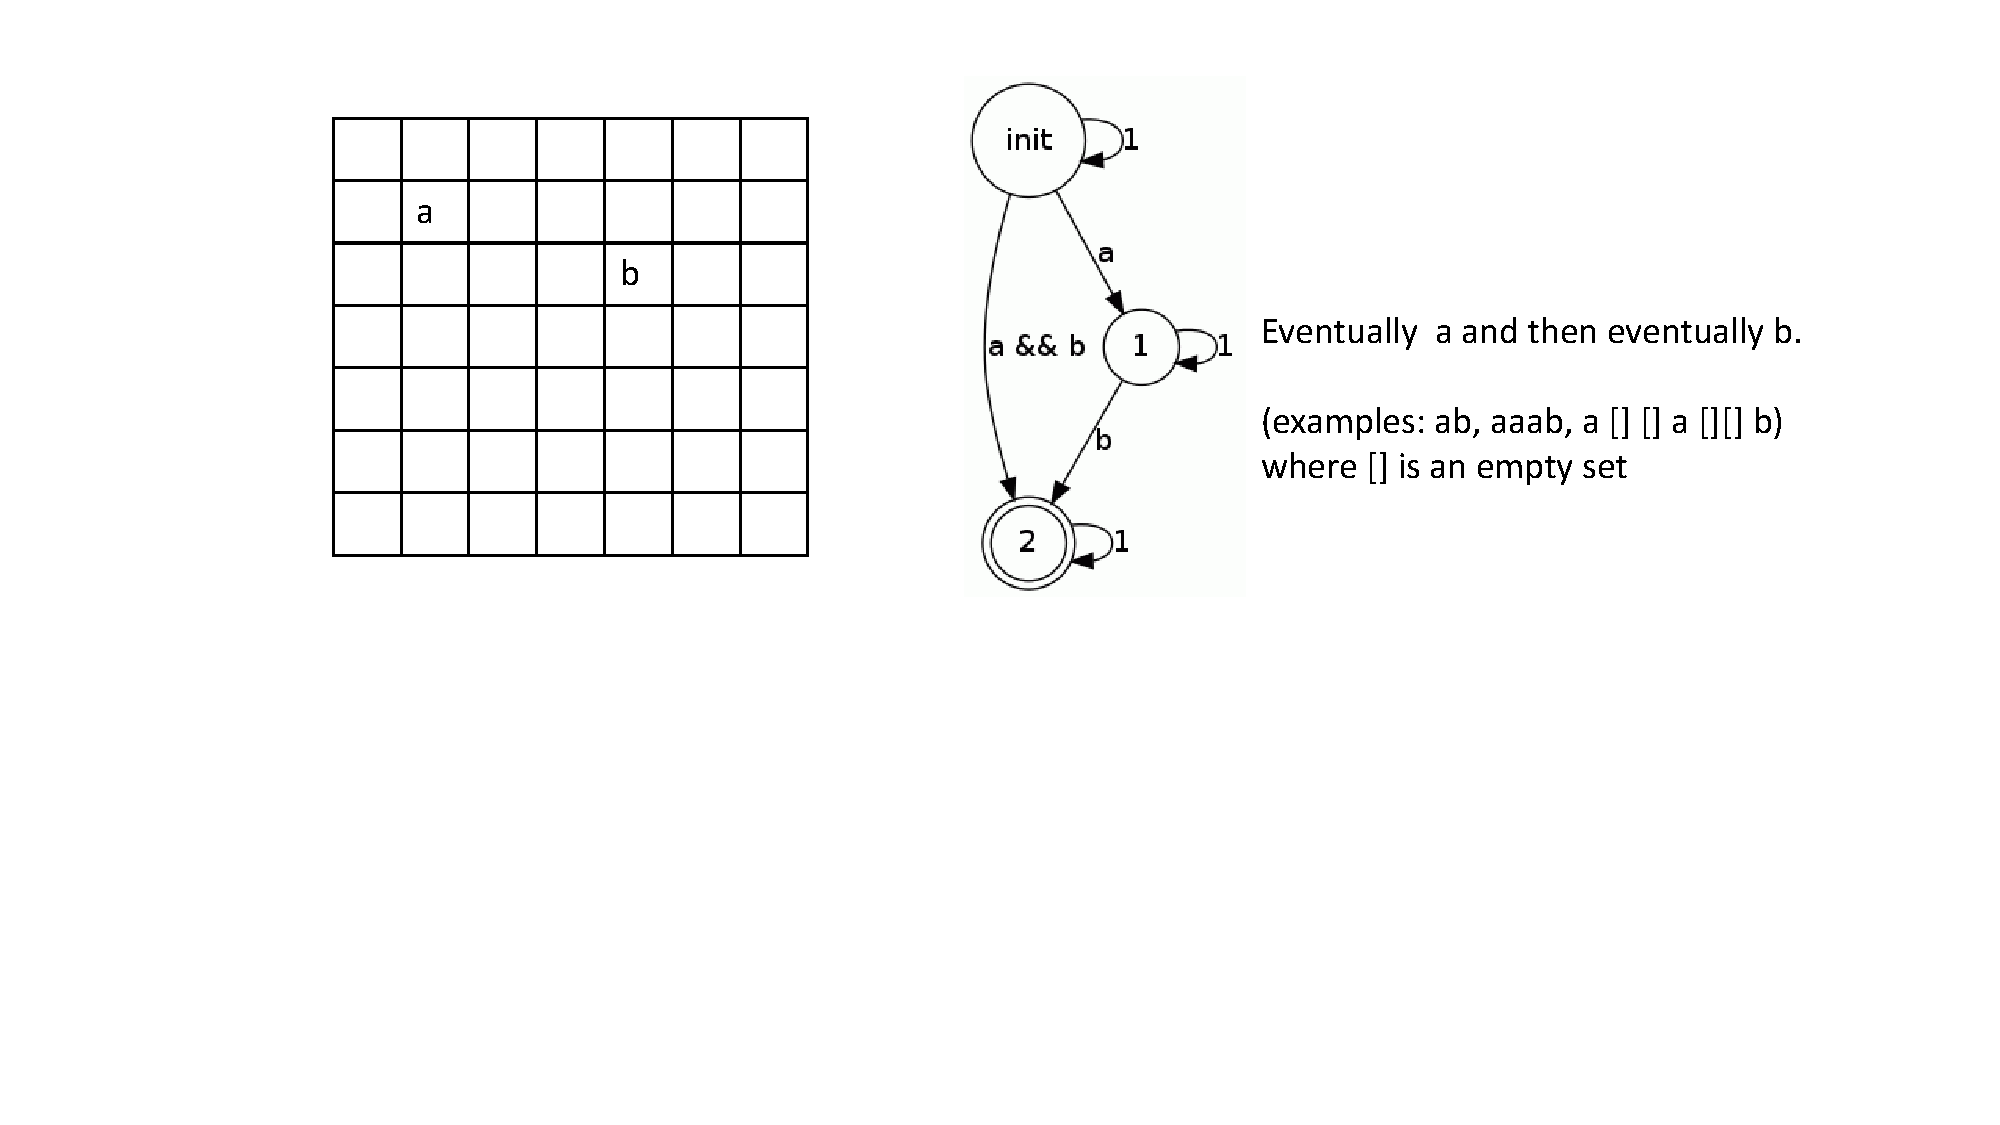
\includegraphics[width=0.9\textwidth]{fig/simpleLTL}
\caption{}
\label{fig:simpleltl}
\end{figure}

Problem 1: Suppose we obtain a set of trajectories, each of which satisfies the
specification. Now, it is of interesting for us to know which reward
function the agent uses.

Problem 2: Suppose a set of agents completing the same tasks but have
different reward functions. Use multi-agent IRL to learn their
respective reward functions and compare the learning result without
using the permissive strategy: Under the same set of features and the
different set of features.

\subsection{Simple case with two-agents}
In the second case, we have more than one agents operates in the same
environment but not at the same time. There are two different
specifications $\varphi_1$ and $\varphi_2$.
$\varphi_1 := \Eventually (a \land \Eventually b)$ and
$\varphi_2 := \Eventually c \lor \Eventually b$. Though two
agents complete totally different tasks, it is not clear whether they
share the same reward function. Note there the reward function
includes additional information for decision making of one agent. For
example, whether agent is concerned about fuel-efficiency (action
cost), or if it is aggrassive in completing the task, or if it is
driven by an interest to visit as much region as possible before
completing the task. 


\subsection{Postive constraint satisfaction: $p < 1$}
Given a formula $\varphi$ and a set of trajectories, we can obtain the
empirical probability of satisfying the specification from the set of
trajectories. This probability is used as $p$. Next, the problem is to
obtain the reward function from the trajectory assuming the constraint
is satisfied at least $p$.


\end{document}
